\documentclass[review]{elsarticle}

\usepackage{lineno,hyperref}
\modulolinenumbers[5]

\journal{Journal of \LaTeX\ Templates}

%%%%%%%%%%%%%%%%%%%%%%%
%% Elsevier bibliography styles
%%%%%%%%%%%%%%%%%%%%%%%
%% To change the style, put a % in front of the second line of the current style and
%% remove the % from the second line of the style you would like to use.
%%%%%%%%%%%%%%%%%%%%%%%

%% Numbered
%\bibliographystyle{model1-num-names}

%% Numbered without titles
%\bibliographystyle{model1a-num-names}

%% Harvard
%\bibliographystyle{model2-names.bst}\biboptions{authoryear}

%% Vancouver numbered
%\usepackage{numcompress}\bibliographystyle{model3-num-names}

%% Vancouver name/year
%\usepackage{numcompress}\bibliographystyle{model4-names}\biboptions{authoryear}

%% APA style
%\bibliographystyle{model5-names}\biboptions{authoryear}

%% AMA style
%\usepackage{numcompress}\bibliographystyle{model6-num-names}

%% `Elsevier LaTeX' style
\bibliographystyle{elsarticle-num}
%%%%%%%%%%%%%%%%%%%%%%%

\begin{document}

\begin{frontmatter}

\title{Positive decadal change in interannual Sea Level variability in the Bay of Bengal}
\tnotetext[mytitlenote]{Fully documented templates are available in the elsarticle package on \href{http://www.ctan.org/tex-archive/macros/latex/contrib/elsarticle}{CTAN}.}

%% Group authors per affiliation:
\author{S. Ghosh\fnref{myfootnote}, A. Mukherjee}
% \address{Radarweg 29, Amsterdam}
% \fntext[myfootnote]{Since 1880.}

%% or include affiliations in footnotes:
% \author[mymainaddress,mysecondaryaddress]{Elsevier Inc}
% \ead[url]{www.elsevier.com}

% \author[mysecondaryaddress]{Global Customer Service\corref{mycorrespondingauthor}}
% \cortext[mycorrespondingauthor]{Corresponding author}
\ead{support@elsevier.com}

% \address[mymainaddress]{1600 John F Kennedy Boulevard, Philadelphia}
% \address[mysecondaryaddress]{360 Park Avenue South, New York}

\begin{abstract}
In this study, we have investigated the decadal change in interannual Sea Level anomaly (SLA) of the Bay of Bengal (BoB) using observed satellite altimeter data and a linear, continuously, and stratified (LCS) model. A rapid increase in SLA during the 2010-19 decade is observed compared to the 2000-09 decade throughout the Spring, Summer, Autumn, and Winter seasons. In order to explain the observed variability, We have executed some numerical experiments using LCS model. The significant change in Ekman pumping and equatorial forcing drives the change in decadal SLA along the western bay of Bengal. The contribution of forcing due to the boundary of the western BoB and Eastern BoB including the Andaman and Nicobar islands is not notable. 
\end{abstract}

\begin{keyword}
\texttt{Sea Lvel Anomaly}\sep Decadal Change 
\MSC[2010] 00-01\sep  99-00
\end{keyword}

\end{frontmatter}

\linenumbers

\section{Introduction}

\section{Data and Model}
\subsection{Observed Data}
We have used daily satellite altimeter observation for the period of 2000-2019 period for our study. The resolution of the satellite altimeter data is 0.25$^o$ x 0.25$^o$. More details can be found from this URL https://cds.climate.copernicus.eu/cdsapp#!/dataset/satellite-sea-level-global?tab=overview . In order to calculate the SLA, we subtracted the long term mean from the daily data.

\subsection{Ocean Model}
In our study, we have used a linear, continuously, stratified (LCS) model to explain the detailed dynamics of SLA, which is a simple wind driven model. The vertical solution of the LCS model is consist of the sum of 10 normal modes, which are estimated based on density profile of \cite{moore1990excitation}. The defined region of this model is from 30$^o$ E-120$^o$E and 30$^o$S-30$^o$N with the horizontal resolution of 0.1$^o$ x 0.1$^o$. In this model, the nonlinear terms like horizontal and vertical advection terms have been not taken into account to maintain the linearity in the model. No slip closed boundary condition has been used in the model.

Land-sea masking of the model is evaluated using the topography of modified Etopo2 (\cite{sindhu2007improved} for the Indian Ocean. Continental shelf regions with the water depth of less than 200 m has been removed from the model. The The Gulf of Mannar area and Pacific ocean has been masked out from the model domain. 

Model simulation has been done for the period of 1991-2019 using ERA5 (\cite{hersbach2020era5}) forcing. The ERA5 data description is available here https://cds.climate.copernicus.eu/cdsapp#!/dataset/reanalysis-era5-single-levels?tab=overview . In this study, model outputs from january 1998 to December 2016 has been used for detailed analysis.


\subsection{Numerical Experiments}
In order to determine the role of different parameters on the SLA, we have done some numerical experiments using the LCS, named as LCSCR, based on previously discussed wind forcing only. There are three types of experiments has been done using the special boundary conditions and linear damper as discussed in \cite{mccreary1996dynamics, mukherjee2017numerical, mukherjee2019signature}. First experiment is related to absence of WBoB local wind by allowing allowing coastal Ekman flow to pass through the boundary using modified no-slip boundary condition ($u_n=v_n=0$) . The modified boundary condition (MBC) is :
\par
$u_n=n.v_n=-n.k * F_n/f$ ;  (1a)
\par
$v_n=k* n.v_n=0$.   (1b)

In the above equation, n is the unit vector normal to the boundary, $F_n$ is the wind-stress vector, k is the unit vector directed upward, f is Coriolis frequency, $u_n$ and $v_n$are velocity components perpendicular and parallel to the boundary. During the first experiment, the above MBC are applied along WBoB ranging from 6.5$^o$N to 20$^o$N. After subtracting the first experiment solution from the LCSCR, we named it LCS$_{WB}$, which represents the influence of WBoB local winds forcing on SLA. Similarly, the second experiment have been done along the eastern and northern boundaries of  BoB including Andaman and Nicobar islands (EBoB)  and after subtracting the solution from the LCSCR solution, we named it LCS$_{EB}$, representing the forcing response only due to above remove coastal winds.

The third experiment has been done using a linear damper between 6.5$^o$N to 6.5$^o$S to stop equatorial wave response to BoB. After subtracting the above solution from the LCSCR, we name it LCS$_{EIO}$, which represents only the influence of equatorial wind on the SLA. And, by subtracting all these three solutions LCS$_{WB}$, LCS$_{EB}$, LCS$_{EIO}$ from the LCSCR, the response from interior BoB is quantified and named as LCS$_{BI}$.   

\subsection{Validation of model}
\cite{shankar2010minima,aparna2012signatures,mukherjee2017numerical,mukherjee2019signature} discussed previously about detailed validation of LCSCR. In this manuscript, we have done a statistical validation of LCSCR in the simulation of altimeter observed SLA in the BoB region. In fig 2, a spatial correlation between observed SLA and LCSCR has been shown and very good correlation (R) values (more than 0.3) have been observed. Also, a good correlation has been observed along the eastern and central parts of BoB with R values greater than 0.4. 


\section{Interannaul SLA variability along WBoB for 2000-09 and 2010-19 decades}
In this section, altimeter observed and LCS model simulated interannual SLA variability during summer season La Nina years between 2000-2019 along WBoB has been discussed. In order to quantify interannual variability of SLA, seasonal variability has been removed using ~400 days low-pass time series 4$'th$ order Butter-worth filter to eliminate the variability associated with less than annual time scale (~400 days).

we have analyzed the decadal changes in the observed interannual SLA in BoB, especially the WBoB. In order to describe interannual variability of SLA along WBoB, regions have been divided into three boxes, which includes northern BoB (NBoB; 85$^o$E-90$^o$E, 17$^o$N,21$^o$N), central BoB (CBoB, 80$^o$E-85$^o$E,14$^o$N-16$^o$N) and southern BoB (SBoB, 80$^o$E-85$^o$E, 10$^o$N-13$^o$N). All three regions are shown in all figures. To specify the decadal variability in BoB SLA, we have subtracted 10 years of SLA climatology of 2000-2009 from SLA climatology of 2010-2019 .



\clearpage
\begin{figure}[!t]
\centering
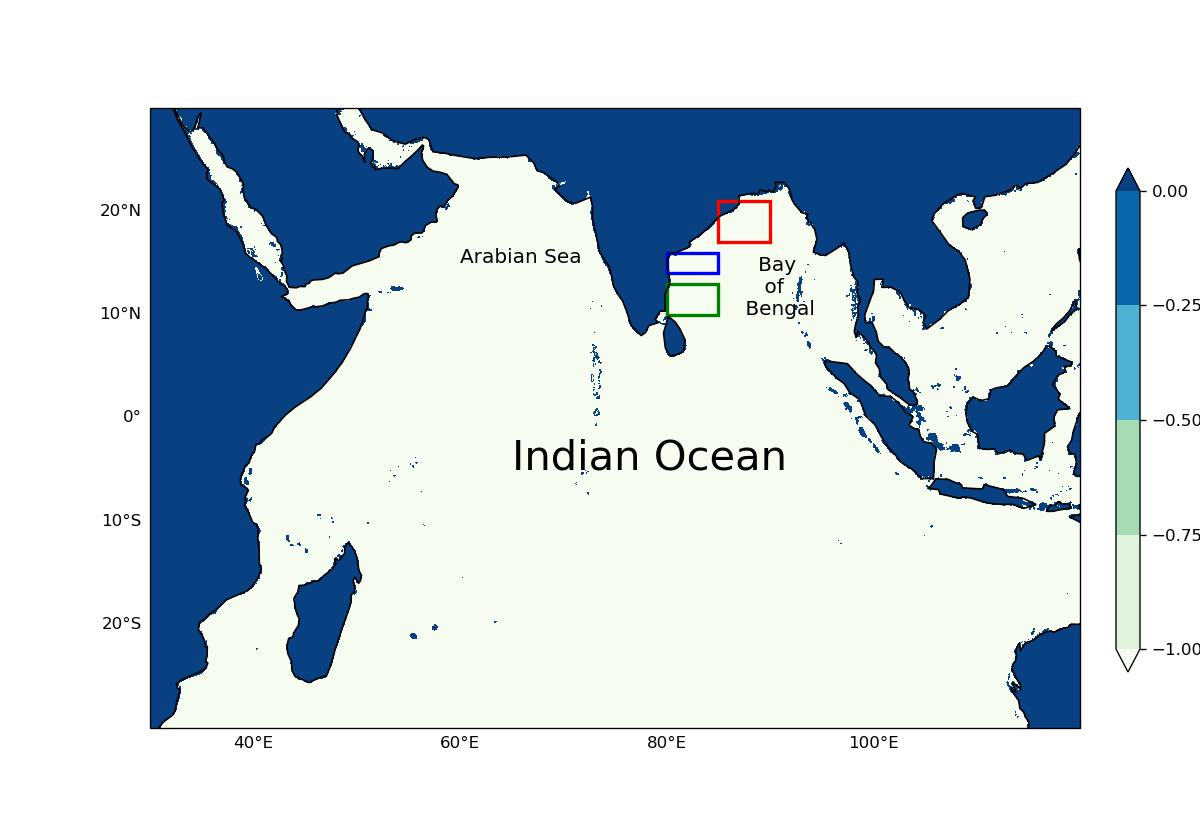
\includegraphics[scale=0.5]{images/domain_fig.jpg}
\caption{}
\label{fig}
\end{figure}

\begin{figure}[!t]
\centering
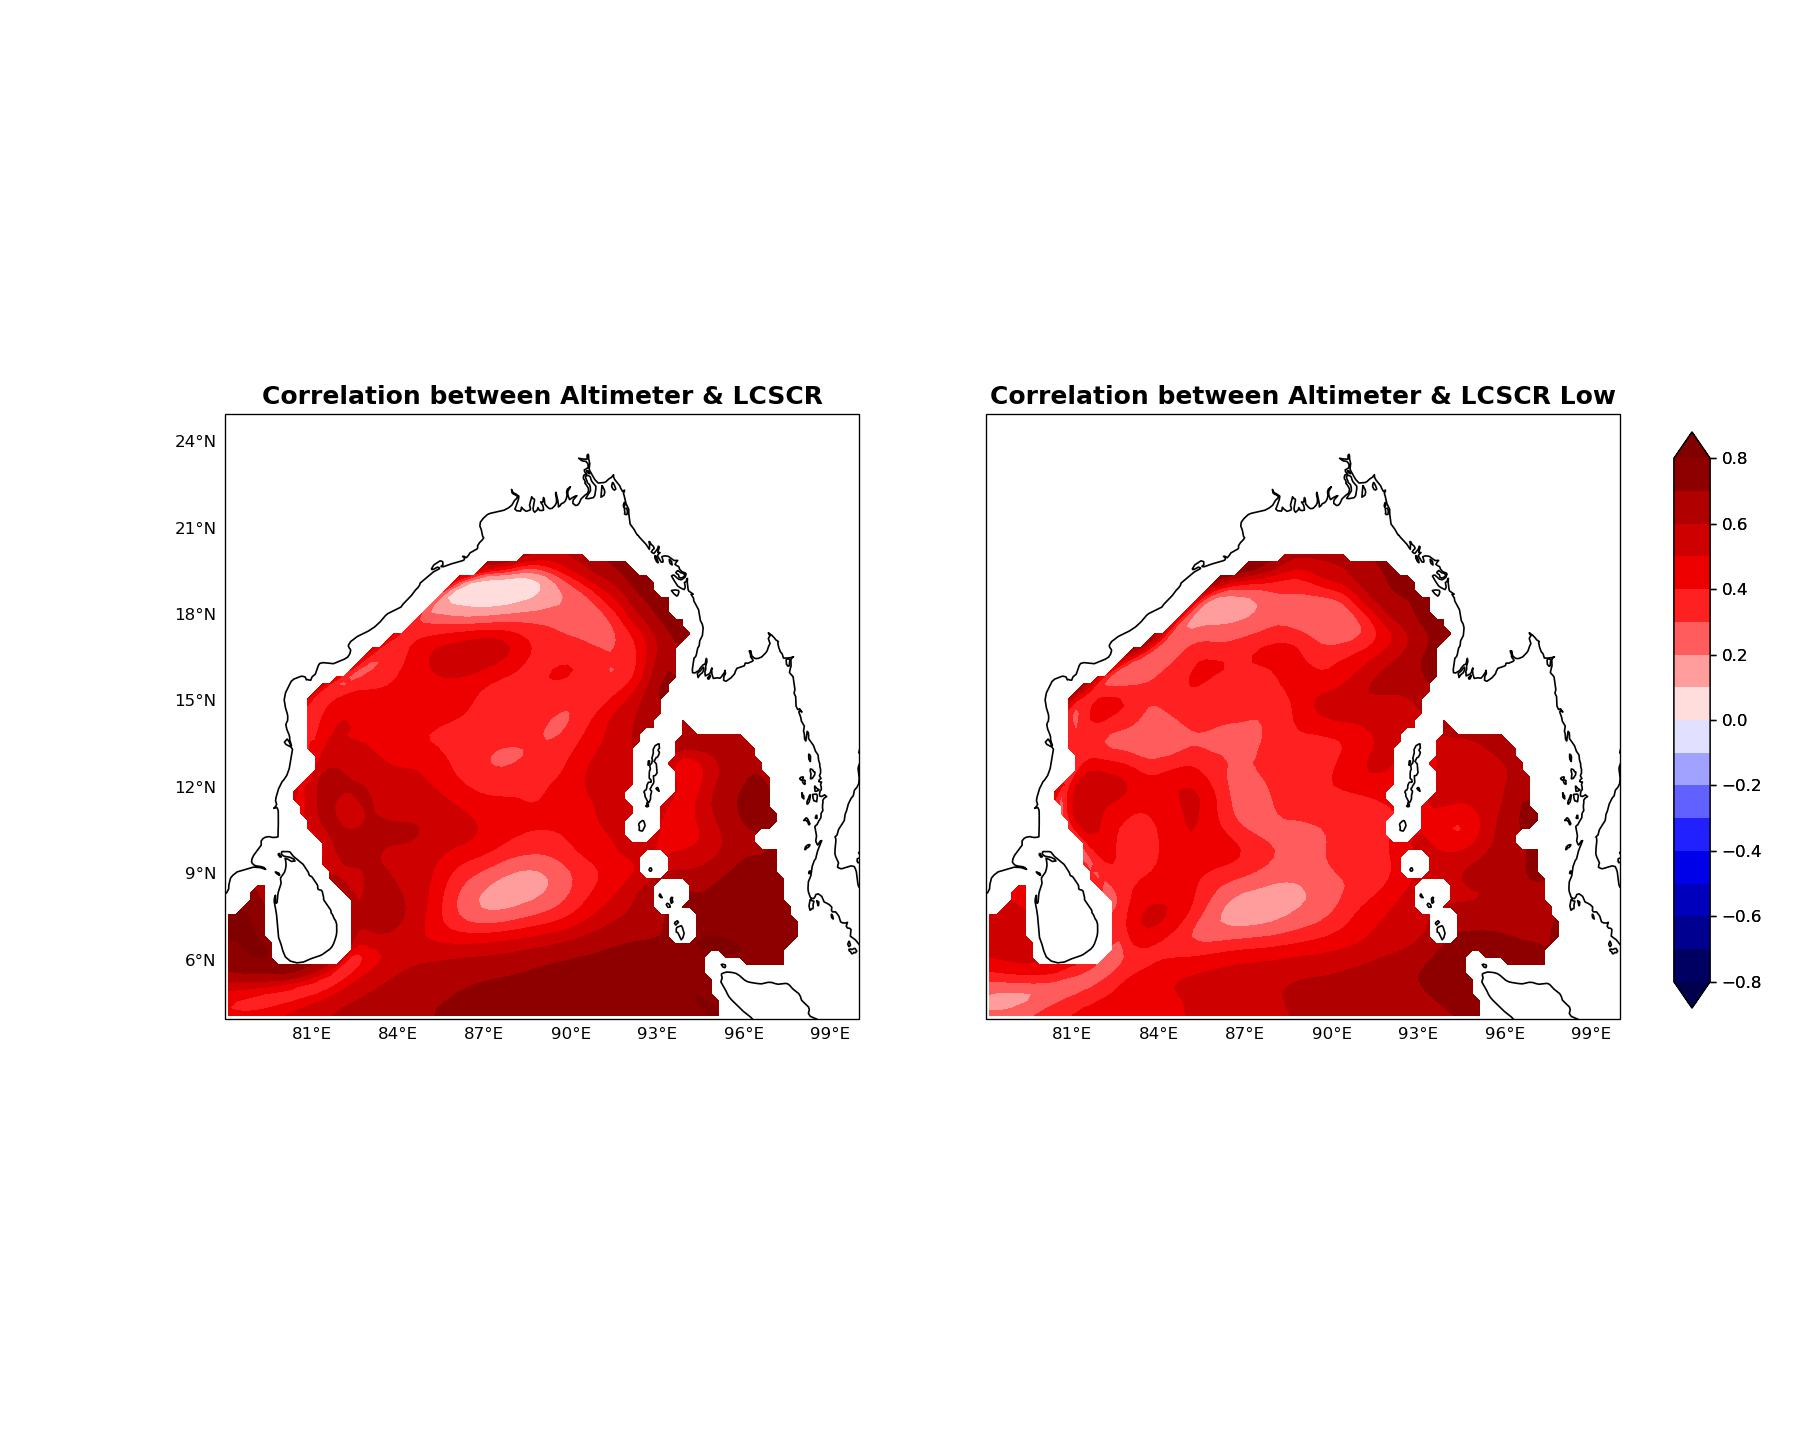
\includegraphics[scale=0.35]{images/corr_plot.jpeg}
\caption{}
\label{fig}
\end{figure}

\begin{figure}[!t]
\centering
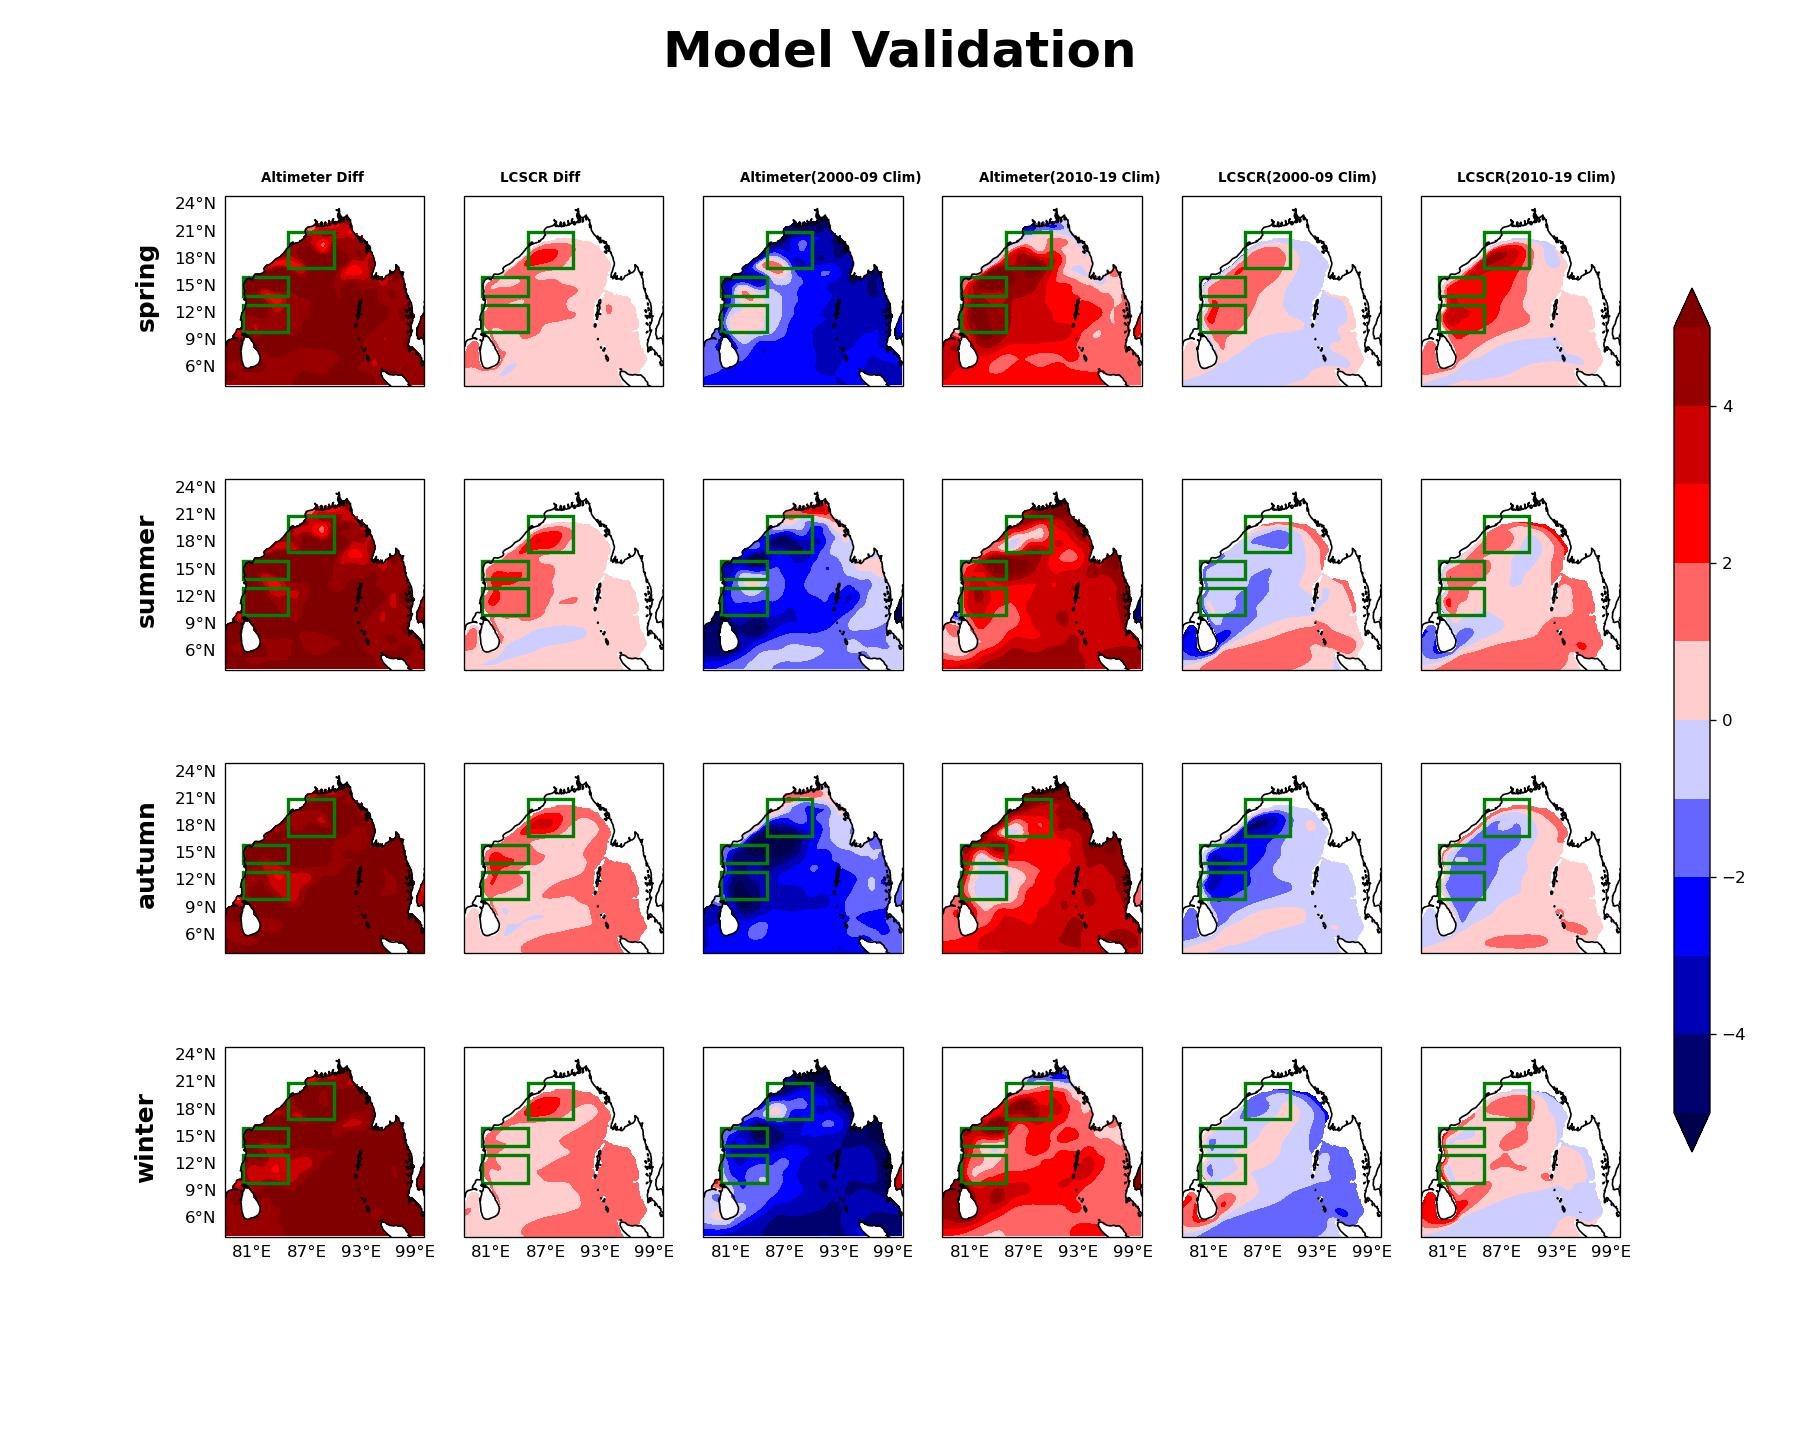
\includegraphics[scale=0.35]{images/validation.jpeg}
\caption{}
\label{fig}
\end{figure}

\begin{figure}[!t]
\centering
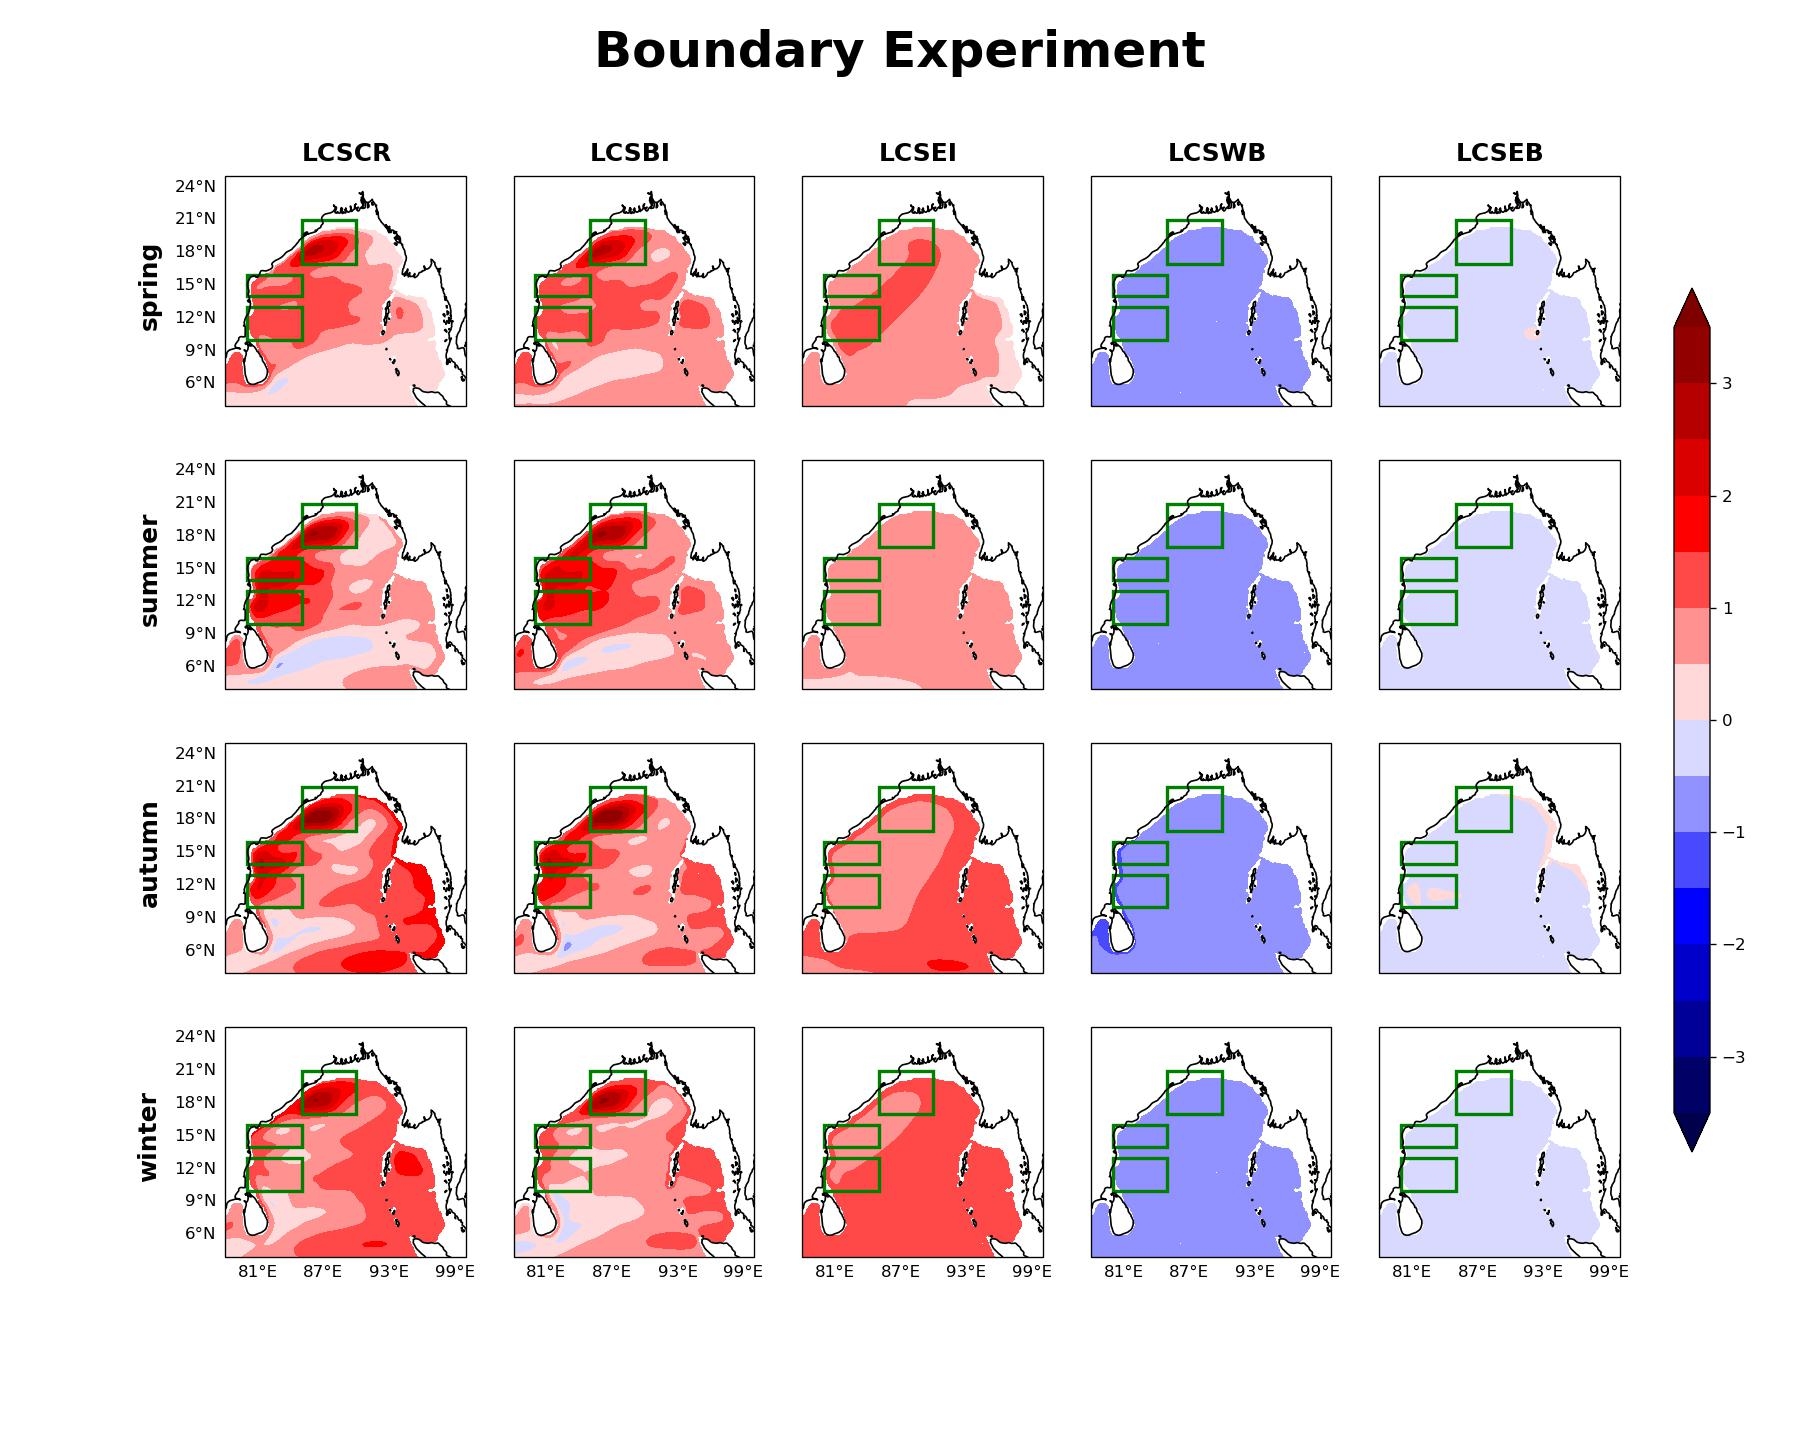
\includegraphics[scale=0.35]{images/boundary_expt.jpeg}
\caption{}
\label{fig}
\end{figure}

\begin{figure}[!t]
\centering
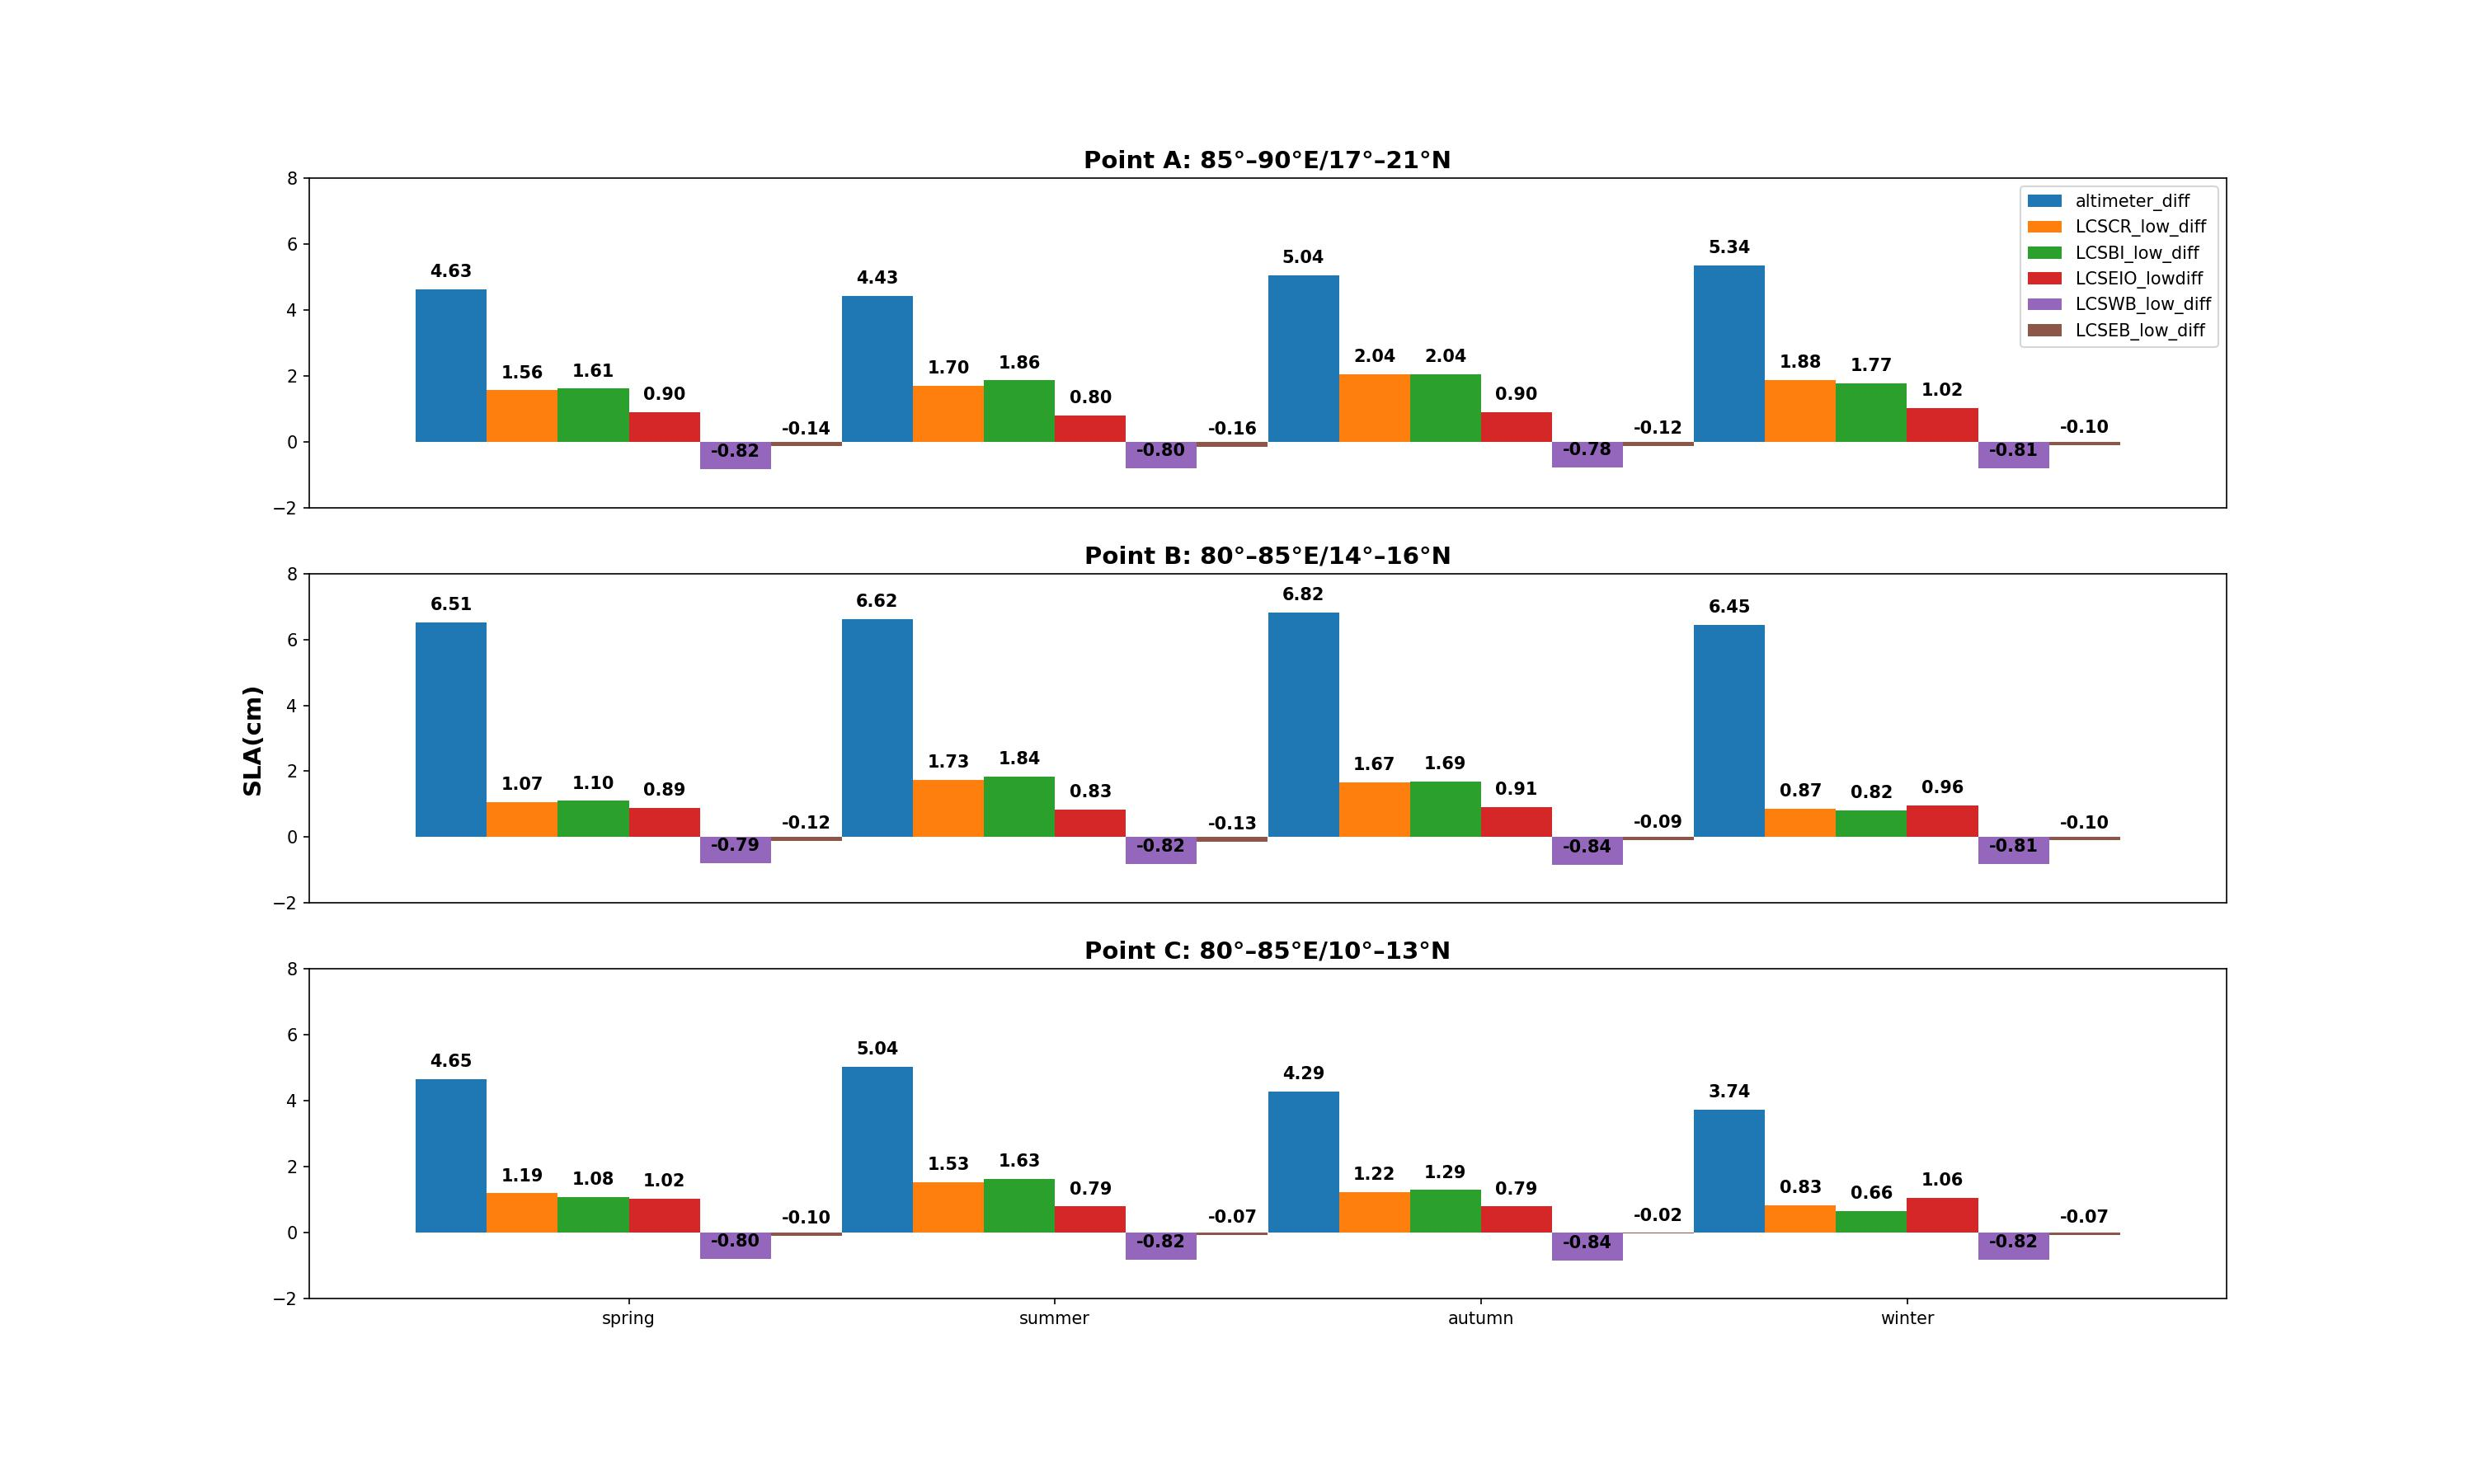
\includegraphics[scale=0.35]{images/point_comparison.jpeg}
\caption{}
\label{fig}
\end{figure}







\bibliography{mybibfile}

\end{document}